\section{Additional performance comparisons}
\label{app:performance_profile}

We provide performance profiles \citep{agarwal2021deep} for \textsc{diamond} and baselines below. % We see that \textsc{diamond} outperforms the baselines in terms of the fraction of runs above a given human normalized score for a range of scores.

%%%%%%%%%%%%%%%%%%%%%%%
\begin{figure}[h!]
\vskip 0.2in
\begin{center}
\centerline{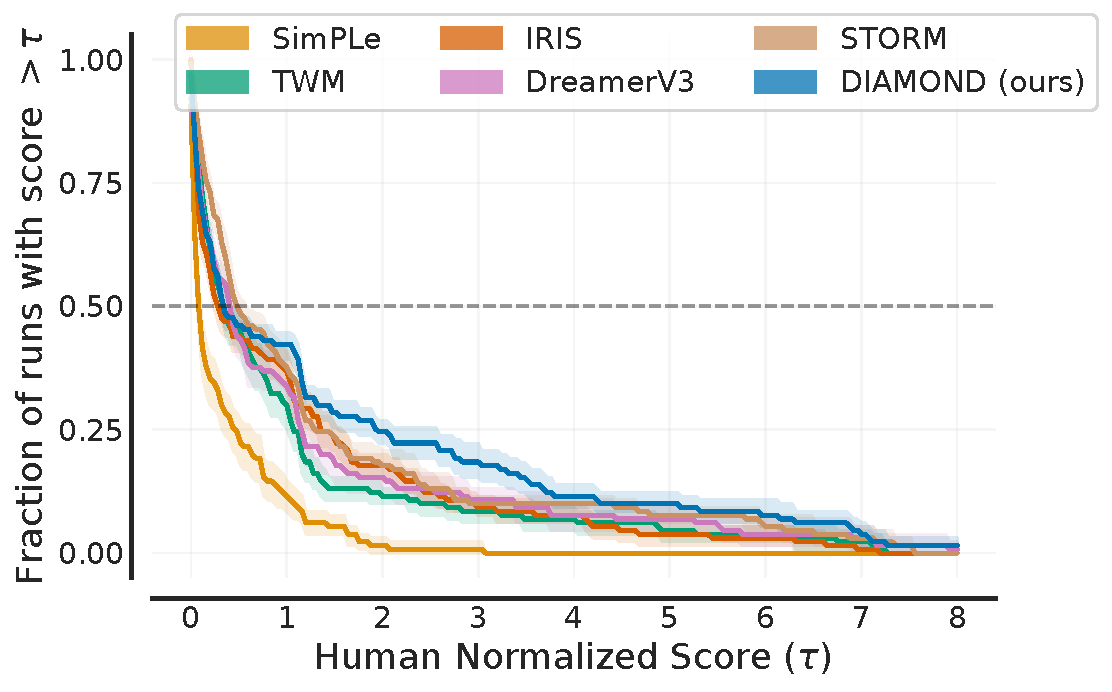
\includegraphics[width=.7\columnwidth]{images/performance_profile.pdf}}
\caption{Performance profiles, i.e. fraction of runs above a given human normalized score.}
\label{fig:results_performance_profile}
\end{center}
\vskip 0.2in
\end{figure}
%%%%%%%%%%%%%%%%%%%%%%%

As additional angles of comparison, we also provide parameter counts and approximate training times for \textsc{iris}, DreamerV3 and \textsc{diamond} in Table \ref{tab:training_time} below. We see that \textsc{diamond} has the highest mean HNS, with fewer parameters than both \textsc{iris} and DreamerV3. \textsc{diamond} also trains faster than \textsc{iris}, although is slower than DreamerV3. 

\begin{table}[h]
\caption{Number of parameters, training time, and mean human-normalized score (HNS).}
\label{tab:training_time}
\begin{center}
\begin{tabular}{lcccc}
\hline
    & \textsc{iris} & DreamerV3 & \textsc{diamond} (ours) & \\ \hline
\#parameters (↓)        & 30M       & 18M            & \textbf{13M}   &  \\
Training days (↓) & 4.1       & \textbf{\textless 1}   & 2.9   &  \\
Mean HNS (↑)            & 1.046     & 1.097          & \textbf{1.459} &  \\ \hline
\end{tabular}
\end{center}
\end{table}



A full training time profile for \textsc{diamond} is provided in Appendix~\ref{app:profiling}.